\documentclass[11pt]{article}
\usepackage{amsmath,amssymb,amsthm}
\usepackage{tikz}
\usetikzlibrary{decorations.pathreplacing,calc,patterns}
\usepackage[margin=1in]{geometry}

\newcommand{\GK}{\operatorname{GK}}
\newcommand{\CPP}{\operatorname{CPP}}

\definecolor{ring1}{RGB}{200,220,255}
\definecolor{ring2}{RGB}{100,150,255}
\definecolor{crushed}{RGB}{220,220,220}

\title{Worked Example: CPP Compression via the ALCD}
\author{Robin Langer}
\date{\today}

\begin{document}
\maketitle

\section{Setup}

Profile $c = (2,1,0)$, $d = 3$.
Consider the CPP $\lambda = \bigl((2),\; (2,1),\; (1)\bigr)$
with $\max(\lambda) = 2$ and $|\lambda| = 6$.

The interlacing chain is
$\nu_1 \xrightarrow{1} \nu_2 \xrightarrow{0} \nu_3 \xrightarrow{2} \nu_1$.


%% ============================================================
\section{The CPP with ring colouring}
%% ============================================================

Each cell in column $j$ of a Young diagram belongs to
\textbf{ring~$j$}.  Peeling ring~$k$ demotes all parts
equal to~$k$ (shortening rows of length~$k$ by one).

\bigskip
\begin{center}
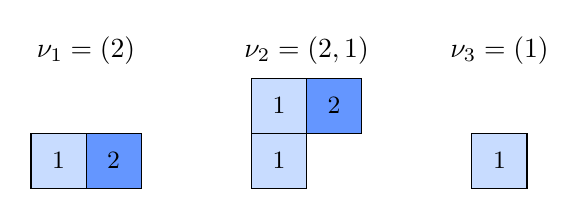
\begin{tikzpicture}[scale=0.7]
  % nu_1 = (2)
  \node at (1, 2.5) {$\nu_1 = (2)$};
  \fill[ring1] (0,0) rectangle (1,1);
  \fill[ring2] (1,0) rectangle (2,1);
  \draw (0,0) grid (2,1);
  \node at (0.5,0.5) {\small 1};
  \node at (1.5,0.5) {\small 2};

  % nu_2 = (2,1)
  \begin{scope}[xshift=4cm]
    \node at (1, 2.5) {$\nu_2 = (2,1)$};
    \fill[ring1] (0,1) rectangle (1,2);
    \fill[ring2] (1,1) rectangle (2,2);
    \fill[ring1] (0,0) rectangle (1,1);
    \draw (0,1) grid (2,2);
    \draw (0,0) grid (1,1);
    \node at (0.5,1.5) {\small 1};
    \node at (1.5,1.5) {\small 2};
    \node at (0.5,0.5) {\small 1};
  \end{scope}

  % nu_3 = (1)
  \begin{scope}[xshift=8cm]
    \node at (0.5, 2.5) {$\nu_3 = (1)$};
    \fill[ring1] (0,0) rectangle (1,1);
    \draw (0,0) grid (1,1);
    \node at (0.5,0.5) {\small 1};
  \end{scope}
\end{tikzpicture}
\end{center}

\noindent
Numbers in cells indicate which ring they belong to.
Light blue = ring~1, dark blue = ring~2.

\medskip\noindent
Face labels (= number of parts demoted per partition):

\smallskip
\begin{center}
\begin{tabular}{c|ccc|c}
Ring $k$ & $b_1$ & $b_2$ & $b_3$ & total \\ \hline
$k=2$ & 1 & 1 & 0 & 2 \\
$k=1$ & 1 & 2 & 1 & 4 \\
\end{tabular}
\end{center}

\noindent
Check: $2 + 4 = 6 = |\lambda|$.



%% ============================================================
\section{The ALCD}
%% ============================================================

The ALCD (growth diagram) records the partitions at each
level and the face labels between consecutive levels.
Peeling proceeds top-down: ring~2 first, then ring~1.

\bigskip
\begin{center}
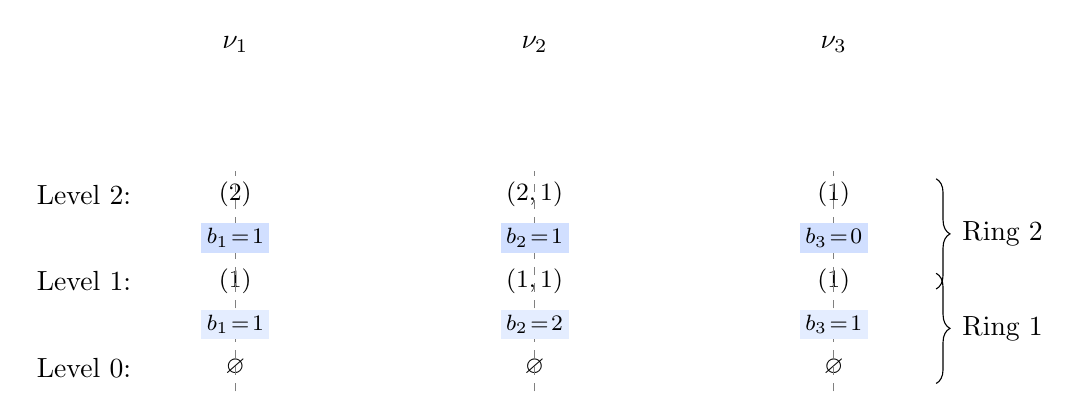
\begin{tikzpicture}[
    level/.style={font=\small},
    face/.style={font=\footnotesize, fill=white, inner sep=2pt},
    >=stealth
  ]
  % Columns
  \def\colsep{3.8}
  \def\rowsep{2.2}

  % Column headers
  \node at (0, 3*\rowsep/2 + 0.8) {$\nu_1$};
  \node at (\colsep, 3*\rowsep/2 + 0.8) {$\nu_2$};
  \node at (2*\colsep, 3*\rowsep/2 + 0.8) {$\nu_3$};

  % Level labels
  \node[left] at (-1.2, 2*\rowsep/2) {Level 2:};
  \node[left] at (-1.2, 1*\rowsep/2) {Level 1:};
  \node[left] at (-1.2, 0) {Level 0:};

  % Level 2 (top) = original CPP
  \node[level] (v1-2) at (0, 2*\rowsep/2) {$(2)$};
  \node[level] (v2-2) at (\colsep, 2*\rowsep/2) {$(2,1)$};
  \node[level] (v3-2) at (2*\colsep, 2*\rowsep/2) {$(1)$};

  % Level 1 = after peeling ring 2
  \node[level] (v1-1) at (0, 1*\rowsep/2) {$(1)$};
  \node[level] (v2-1) at (\colsep, 1*\rowsep/2) {$(1,1)$};
  \node[level] (v3-1) at (2*\colsep, 1*\rowsep/2) {$(1)$};

  % Level 0 = empty
  \node[level] (v1-0) at (0, 0) {$\varnothing$};
  \node[level] (v2-0) at (\colsep, 0) {$\varnothing$};
  \node[level] (v3-0) at (2*\colsep, 0) {$\varnothing$};

  % Vertical lines
  \foreach \j in {0,1,2} {
    \draw[gray,dashed] (\j*\colsep, -0.3) -- (\j*\colsep, 2*\rowsep/2+0.3);
  }

  % Ring 2 face labels (between level 2 and level 1)
  \node[face, fill=ring2!30] at (0, 1.5*\rowsep/2) {$b_1\!=\!1$};
  \node[face, fill=ring2!30] at (\colsep, 1.5*\rowsep/2) {$b_2\!=\!1$};
  \node[face, fill=ring2!30] at (2*\colsep, 1.5*\rowsep/2) {$b_3\!=\!0$};

  % Ring 1 face labels (between level 1 and level 0)
  \node[face, fill=ring1!50] at (0, 0.5*\rowsep/2) {$b_1\!=\!1$};
  \node[face, fill=ring1!50] at (\colsep, 0.5*\rowsep/2) {$b_2\!=\!2$};
  \node[face, fill=ring1!50] at (2*\colsep, 0.5*\rowsep/2) {$b_3\!=\!1$};

  % Ring labels on the right
  \draw[decorate, decoration={brace, amplitude=5pt}]
    (2*\colsep+1.3, 2*\rowsep/2+0.2) -- (2*\colsep+1.3, \rowsep/2-0.1)
    node[midway, right=6pt] {Ring 2};
  \draw[decorate, decoration={brace, amplitude=5pt}]
    (2*\colsep+1.3, \rowsep/2+0.1) -- (2*\colsep+1.3, -0.2)
    node[midway, right=6pt] {Ring 1};
\end{tikzpicture}
\end{center}


%% ============================================================
\section{Four compressions of $\lambda$}
%% ============================================================

A \emph{compression} selects a subset $S \subseteq \{1,\ldots,n\}$
of rings to \textbf{crush} (remove entirely).  The remaining
rings form a residual CPP $\mu$ with
$\max(\mu) = n - |S|$.  The sign is $(-1)^{|S|}$ and the
total weight is $\sigma(S) + |\mu|$.

\bigskip

%%% --- Compression (a): S = empty ---
\noindent\textbf{(a)} $S = \varnothing$: keep all rings.

\smallskip
\begin{center}
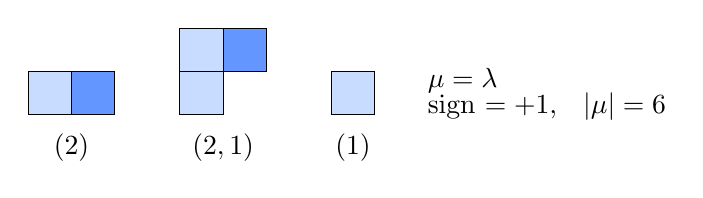
\begin{tikzpicture}[scale=0.55]
  % nu_1
  \fill[ring1] (0,0) rectangle (1,1);
  \fill[ring2] (1,0) rectangle (2,1);
  \draw (0,0) grid (2,1);
  \node[below] at (1,-0.2) {$(2)$};
  % nu_2
  \begin{scope}[xshift=3.5cm]
    \fill[ring1] (0,1) rectangle (1,2);
    \fill[ring2] (1,1) rectangle (2,2);
    \fill[ring1] (0,0) rectangle (1,1);
    \draw (0,1) grid (2,2);
    \draw (0,0) grid (1,1);
    \node[below] at (1,-0.2) {$(2,1)$};
  \end{scope}
  % nu_3
  \begin{scope}[xshift=7cm]
    \fill[ring1] (0,0) rectangle (1,1);
    \draw (0,0) grid (1,1);
    \node[below] at (0.5,-0.2) {$(1)$};
  \end{scope}
  % Label
  \node[right] at (9, 0.8) {$\mu = \lambda$};
  \node[right] at (9, 0.2) {sign $= +1$, \; $|\mu| = 6$};
\end{tikzpicture}
\end{center}

\bigskip

%%% --- Compression (b): S = {2} ---
\noindent\textbf{(b)} $S = \{2\}$: crush ring~2 (outermost).

\smallskip
\begin{center}
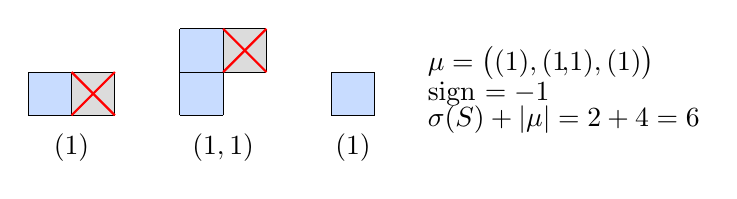
\begin{tikzpicture}[scale=0.55]
  % nu_1 = (1)
  \fill[ring1] (0,0) rectangle (1,1);
  \fill[crushed] (1,0) rectangle (2,1);
  \draw (0,0) grid (2,1);
  \draw[red, thick] (1,0) -- (2,1);
  \draw[red, thick] (1,1) -- (2,0);
  \node[below] at (1,-0.2) {$(1)$};
  % nu_2
  \begin{scope}[xshift=3.5cm]
    \fill[ring1] (0,1) rectangle (1,2);
    \fill[crushed] (1,1) rectangle (2,2);
    \fill[ring1] (0,0) rectangle (1,1);
    \draw (0,1) grid (2,2);
    \draw (0,0) grid (1,1);
    \draw[red, thick] (1,1) -- (2,2);
    \draw[red, thick] (1,2) -- (2,1);
    \node[below] at (1,-0.2) {$(1,1)$};
  \end{scope}
  % nu_3
  \begin{scope}[xshift=7cm]
    \fill[ring1] (0,0) rectangle (1,1);
    \draw (0,0) grid (1,1);
    \node[below] at (0.5,-0.2) {$(1)$};
  \end{scope}
  % Label
  \node[right] at (9, 1.2) {$\mu = \bigl((1),(1\!,\!1),(1)\bigr)$};
  \node[right] at (9, 0.5) {sign $= -1$};
  \node[right] at (9, -0.1) {$\sigma(S) + |\mu| = 2 + 4 = 6$};
\end{tikzpicture}
\end{center}

\bigskip

%%% --- Compression (c): S = {1} ---
\noindent\textbf{(c)} $S = \{1\}$: crush ring~1 (innermost).

\smallskip
\begin{center}
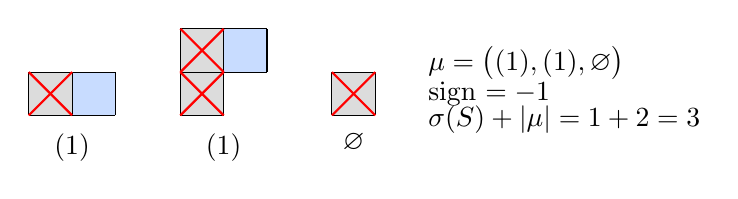
\begin{tikzpicture}[scale=0.55]
  % nu_1: ring 1 crushed, ring 2 remains (renumbered to ring 1)
  \fill[crushed] (0,0) rectangle (1,1);
  \fill[ring1] (1,0) rectangle (2,1);
  \draw (0,0) grid (2,1);
  \draw[red, thick] (0,0) -- (1,1);
  \draw[red, thick] (0,1) -- (1,0);
  \node[below] at (1,-0.2) {$(1)$};
  % nu_2
  \begin{scope}[xshift=3.5cm]
    \fill[crushed] (0,1) rectangle (1,2);
    \fill[ring1] (1,1) rectangle (2,2);
    \fill[crushed] (0,0) rectangle (1,1);
    \draw (0,1) grid (2,2);
    \draw (0,0) grid (1,1);
    \draw[red, thick] (0,1) -- (1,2);
    \draw[red, thick] (0,2) -- (1,1);
    \draw[red, thick] (0,0) -- (1,1);
    \draw[red, thick] (0,1) -- (1,0);
    \node[below] at (1,-0.2) {$(1)$};
  \end{scope}
  % nu_3: ring 1 crushed, nothing from ring 2
  \begin{scope}[xshift=7cm]
    \fill[crushed] (0,0) rectangle (1,1);
    \draw (0,0) grid (1,1);
    \draw[red, thick] (0,0) -- (1,1);
    \draw[red, thick] (0,1) -- (1,0);
    \node[below] at (0.5,-0.2) {$\varnothing$};
  \end{scope}
  % Label
  \node[right] at (9, 1.2) {$\mu = \bigl((1),(1),\varnothing\bigr)$};
  \node[right] at (9, 0.5) {sign $= -1$};
  \node[right] at (9, -0.1) {$\sigma(S) + |\mu| = 1 + 2 = 3$};
\end{tikzpicture}
\end{center}

\bigskip

%%% --- Compression (d): S = {1,2} ---
\noindent\textbf{(d)} $S = \{1,2\}$: crush both rings.

\smallskip
\begin{center}
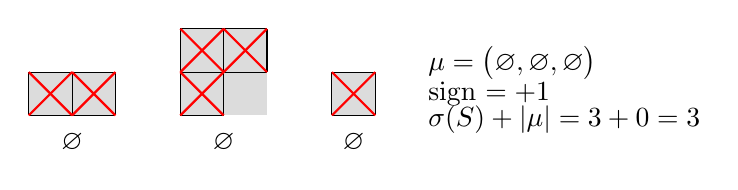
\begin{tikzpicture}[scale=0.55]
  % All crushed
  \fill[crushed] (0,0) rectangle (2,1);
  \draw (0,0) grid (2,1);
  \draw[red, thick] (0,0) -- (1,1);
  \draw[red, thick] (0,1) -- (1,0);
  \draw[red, thick] (1,0) -- (2,1);
  \draw[red, thick] (1,1) -- (2,0);
  \node[below] at (1,-0.2) {$\varnothing$};
  % nu_2
  \begin{scope}[xshift=3.5cm]
    \fill[crushed] (0,0) rectangle (2,2);
    \fill[crushed] (0,0) rectangle (1,1);
    \draw (0,1) grid (2,2);
    \draw (0,0) grid (1,1);
    \draw[red, thick] (0,1) -- (1,2);
    \draw[red, thick] (0,2) -- (1,1);
    \draw[red, thick] (1,1) -- (2,2);
    \draw[red, thick] (1,2) -- (2,1);
    \draw[red, thick] (0,0) -- (1,1);
    \draw[red, thick] (0,1) -- (1,0);
    \node[below] at (1,-0.2) {$\varnothing$};
  \end{scope}
  % nu_3
  \begin{scope}[xshift=7cm]
    \fill[crushed] (0,0) rectangle (1,1);
    \draw (0,0) grid (1,1);
    \draw[red, thick] (0,0) -- (1,1);
    \draw[red, thick] (0,1) -- (1,0);
    \node[below] at (0.5,-0.2) {$\varnothing$};
  \end{scope}
  % Label
  \node[right] at (9, 1.2) {$\mu = \bigl(\varnothing,\varnothing,\varnothing\bigr)$};
  \node[right] at (9, 0.5) {sign $= +1$};
  \node[right] at (9, -0.1) {$\sigma(S) + |\mu| = 3 + 0 = 3$};
\end{tikzpicture}
\end{center}


%% ============================================================
\section{Cancellation}
%% ============================================================

The four compressions of $\lambda$ produce ground-set
elements at two different total weights:

\medskip
\begin{center}
\begin{tabular}{c|c|c|c|c}
  & $S$ & $\mu$ & sign & total weight \\ \hline
(a) & $\varnothing$ & $\lambda$ & $+1$ & $6$ \\
(b) & $\{2\}$ & $\bigl((1),(1\!,\!1),(1)\bigr)$ & $-1$ & $6$ \\[4pt]
(c) & $\{1\}$ & $\bigl((1),(1),\varnothing\bigr)$ & $-1$ & $3$ \\
(d) & $\{1,2\}$ & $\bigl(\varnothing,\varnothing,\varnothing\bigr)$ & $+1$ & $3$ \\
\end{tabular}
\end{center}

\medskip\noindent
At weight~6: (a) has sign $+1$, (b) has sign $-1$.
They cancel.

\noindent
At weight~3: (d) has sign $+1$, (c) has sign $-1$.
They cancel.

\medskip\noindent
\textbf{Every compression of $\lambda$ cancels with a
partner at the same total weight and opposite sign.}

\medskip\noindent
The conjecture $Q_n \in \mathbb{N}[q]$ asserts that this
cancellation holds globally: across all CPPs and all
compressions, the positive terms outweigh the negative
ones at every power of~$q$.


%% ============================================================
\section{The ALCD viewpoint}
%% ============================================================

The four compressions correspond to four ways of
\emph{slicing} the ALCD:

\bigskip
\begin{center}
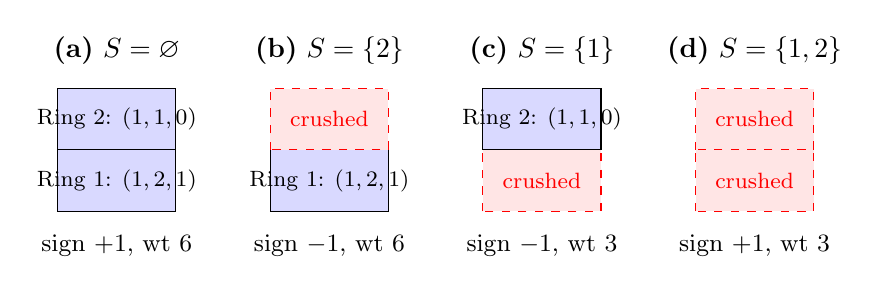
\begin{tikzpicture}[scale=0.6,
    kept/.style={fill=blue!15, draw=black},
    crush/.style={fill=red!10, draw=red, dashed},
    label/.style={font=\footnotesize}
  ]
  \def\w{2.5}
  \def\h{1.3}

  % --- (a) Keep both ---
  \begin{scope}[xshift=0cm]
    \node[above] at (\w/2, 2*\h+0.3) {\textbf{(a)} $S=\varnothing$};
    \draw[kept] (0,0) rectangle (\w,\h);
    \draw[kept] (0,\h) rectangle (\w,2*\h);
    \node[label] at (\w/2, 0.5*\h) {Ring 1: $(1,2,1)$};
    \node[label] at (\w/2, 1.5*\h) {Ring 2: $(1,1,0)$};
    \node[below, font=\small] at (\w/2, -0.3) {sign $+1$, wt $6$};
  \end{scope}

  % --- (b) Crush ring 2 ---
  \begin{scope}[xshift=4.5cm]
    \node[above] at (\w/2, 2*\h+0.3) {\textbf{(b)} $S=\{2\}$};
    \draw[kept] (0,0) rectangle (\w,\h);
    \draw[crush] (0,\h) rectangle (\w,2*\h);
    \node[label] at (\w/2, 0.5*\h) {Ring 1: $(1,2,1)$};
    \node[label, red] at (\w/2, 1.5*\h) {crushed};
    \node[below, font=\small] at (\w/2, -0.3) {sign $-1$, wt $6$};
  \end{scope}

  % --- (c) Crush ring 1 ---
  \begin{scope}[xshift=9cm]
    \node[above] at (\w/2, 2*\h+0.3) {\textbf{(c)} $S=\{1\}$};
    \draw[crush] (0,0) rectangle (\w,\h);
    \draw[kept] (0,\h) rectangle (\w,2*\h);
    \node[label, red] at (\w/2, 0.5*\h) {crushed};
    \node[label] at (\w/2, 1.5*\h) {Ring 2: $(1,1,0)$};
    \node[below, font=\small] at (\w/2, -0.3) {sign $-1$, wt $3$};
  \end{scope}

  % --- (d) Crush both ---
  \begin{scope}[xshift=13.5cm]
    \node[above] at (\w/2, 2*\h+0.3) {\textbf{(d)} $S=\{1,2\}$};
    \draw[crush] (0,0) rectangle (\w,\h);
    \draw[crush] (0,\h) rectangle (\w,2*\h);
    \node[label, red] at (\w/2, 0.5*\h) {crushed};
    \node[label, red] at (\w/2, 1.5*\h) {crushed};
    \node[below, font=\small] at (\w/2, -0.3) {sign $+1$, wt $3$};
  \end{scope}
\end{tikzpicture}
\end{center}

\medskip\noindent
Crushing a ring changes the sign (by $(-1)$) and adds
the ring index to the total weight (via $\sigma(S)$),
while removing that ring's contribution $|\mu|$ decreases.
The net effect: crushing ring~$k$ changes the total weight
by $k - (\text{weight of ring } k)$.

\medskip\noindent
Specifically:
\begin{itemize}
  \item Crushing ring~2 changes weight by
    $+2 - 2 = 0$ (weight preserved).
  \item Crushing ring~1 changes weight by
    $+1 - 4 = -3$ (weight decreases by~3).
\end{itemize}

\noindent
Compressions (a) and (b) are at the \emph{same} weight
because ring~2's face-label total equals its index.
This is the key condition for a weight-preserving
sign-reversing pairing.


%% ============================================================
\section{Including $U$: the full ground set}
%% ============================================================

The previous sections used $U = \varnothing$.  The full
ground-set element is a triple $(S, U, \mu)$ where:
\begin{itemize}
  \item $S \subseteq \{1, \ldots, n\}$ --- crushed rings
    (from the Euler product $(zq;q)_\infty$).
  \item $\mu$ --- residual CPP with $\max(\mu) = m := n - |S|$.
  \item $U \subseteq \{1, \ldots, m\}$ --- \textbf{marked rings}
    of $\mu$ (from the Pochhammer $(q)_m$).
\end{itemize}
The sign is $(-1)^{|S| + |U|}$ and the total weight is
$\sigma(S) + \sigma(U) + |\mu|$.

\medskip\noindent
The Pochhammer factor
$(q)_m = \prod_{k=1}^{m}(1 - q^k)$
expands as
\[
  (q)_m = \sum_{U \subseteq \{1,\ldots,m\}} (-1)^{|U|}\, q^{\sigma(U)}.
\]
Each subset $U$ ``marks'' certain rings of $\mu$.
Marking ring~$k$ flips the sign and adds $k$ to the weight.


\subsection*{Full table from $\lambda = \bigl((2),(2,1),(1)\bigr)$}

With $U$ included, a single CPP generates many more
ground-set elements:

\medskip
\begin{center}
\renewcommand{\arraystretch}{1.2}
\begin{tabular}{c|c|c|c|c|c}
  & $S$ & $U$ & $\mu$ & sign & total wt \\ \hline
1 & $\varnothing$ & $\varnothing$ & $\lambda$ & $+$ & $6$ \\
2 & $\{2\}$ & $\varnothing$ &
  $\bigl((1),(1\!,\!1),(1)\bigr)$ & $-$ & $6$ \\[3pt] \hline
3 & $\varnothing$ & $\{1\}$ & $\lambda$ & $-$ & $7$ \\
4 & $\{2\}$ & $\{1\}$ &
  $\bigl((1),(1\!,\!1),(1)\bigr)$ & $+$ & $7$ \\[3pt] \hline
5 & $\varnothing$ & $\{2\}$ & $\lambda$ & $-$ & $8$ \\[3pt] \hline
6 & $\varnothing$ & $\{1,2\}$ & $\lambda$ & $+$ & $9$ \\[3pt]
  \hline\hline
7 & $\{1\}$ & $\varnothing$ &
  $\bigl((1),(1),\varnothing\bigr)$ & $-$ & $3$ \\
8 & $\{1,2\}$ & $\varnothing$ &
  $\bigl(\varnothing,\varnothing,\varnothing\bigr)$ & $+$ & $3$
  \\[3pt] \hline
9 & $\{1\}$ & $\{1\}$ &
  $\bigl((1),(1),\varnothing\bigr)$ & $+$ & $4$ \\
\end{tabular}
\end{center}

\medskip\noindent
\textbf{Cancellation within this CPP:}
\begin{itemize}
  \item Rows 1 \& 2 cancel at weight~6
    ($S = \varnothing$ vs $S = \{2\}$, same $U = \varnothing$).
  \item Rows 3 \& 4 cancel at weight~7
    ($S = \varnothing$ vs $S = \{2\}$, same $U = \{1\}$).
  \item Rows 7 \& 8 cancel at weight~3
    ($S = \{1\}$ vs $S = \{1,2\}$, same $U = \varnothing$).
\end{itemize}

\noindent
\textbf{Survivors from this CPP:}
\begin{itemize}
  \item Row 5: sign $-$, weight~8.
    Needs a partner from a \emph{different} CPP.
  \item Row 6: sign $+$, weight~9.
    Needs a partner from a different CPP.
  \item Row 9: sign $+$, weight~4.
    Needs a partner from a different CPP.
\end{itemize}

\subsection*{ALCD with $U$-marking}

Visually, $U$ marks rings \emph{within} the residual
$\mu$.  Marked rings are shown with a star.

\bigskip
\begin{center}
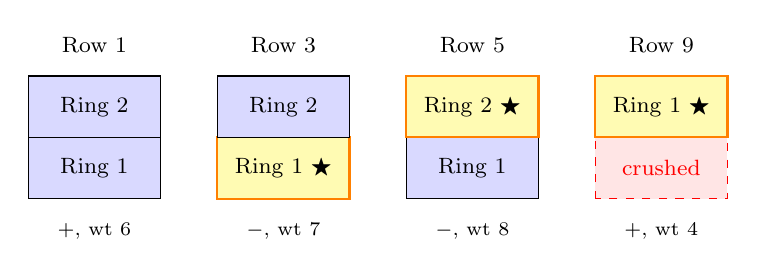
\begin{tikzpicture}[scale=0.6,
    kept/.style={fill=blue!15, draw=black},
    crush/.style={fill=red!10, draw=red, dashed},
    marked/.style={fill=yellow!30, draw=black,
      postaction={draw, thick, orange}},
    label/.style={font=\footnotesize}
  ]
  \def\w{2.8}
  \def\h{1.3}

  % --- Row 1: S=empty, U=empty ---
  \begin{scope}[xshift=0cm]
    \node[above] at (\w/2, 2*\h+0.3)
      {\footnotesize Row 1};
    \draw[kept] (0,0) rectangle (\w,\h);
    \draw[kept] (0,\h) rectangle (\w,2*\h);
    \node[label] at (\w/2, 0.5*\h) {Ring 1};
    \node[label] at (\w/2, 1.5*\h) {Ring 2};
    \node[below, font=\scriptsize] at (\w/2, -0.3)
      {$+$, wt $6$};
  \end{scope}

  % --- Row 3: S=empty, U={1} ---
  \begin{scope}[xshift=4cm]
    \node[above] at (\w/2, 2*\h+0.3)
      {\footnotesize Row 3};
    \draw[marked] (0,0) rectangle (\w,\h);
    \draw[kept] (0,\h) rectangle (\w,2*\h);
    \node[label] at (\w/2, 0.5*\h) {Ring 1 $\bigstar$};
    \node[label] at (\w/2, 1.5*\h) {Ring 2};
    \node[below, font=\scriptsize] at (\w/2, -0.3)
      {$-$, wt $7$};
  \end{scope}

  % --- Row 5: S=empty, U={2} ---
  \begin{scope}[xshift=8cm]
    \node[above] at (\w/2, 2*\h+0.3)
      {\footnotesize Row 5};
    \draw[kept] (0,0) rectangle (\w,\h);
    \draw[marked] (0,\h) rectangle (\w,2*\h);
    \node[label] at (\w/2, 0.5*\h) {Ring 1};
    \node[label] at (\w/2, 1.5*\h) {Ring 2 $\bigstar$};
    \node[below, font=\scriptsize] at (\w/2, -0.3)
      {$-$, wt $8$};
  \end{scope}

  % --- Row 9: S={1}, U={1} ---
  \begin{scope}[xshift=12cm]
    \node[above] at (\w/2, 2*\h+0.3)
      {\footnotesize Row 9};
    \draw[crush] (0,0) rectangle (\w,\h);
    \draw[marked] (0,\h) rectangle (\w,2*\h);
    \node[label, red] at (\w/2, 0.5*\h) {crushed};
    \node[label] at (\w/2, 1.5*\h) {Ring 1 $\bigstar$};
    \node[below, font=\scriptsize] at (\w/2, -0.3)
      {$+$, wt $4$};
  \end{scope}
\end{tikzpicture}
\end{center}

\medskip\noindent
Three operations on the ALCD, each flipping the sign:
\begin{enumerate}
  \item \textbf{Crush} a ring (move index from
    $\mu$ to $S$): adds $k$ to $\sigma(S)$, removes
    ring~$k$'s weight from $|\mu|$.
  \item \textbf{Mark} a ring (add index to $U$):
    adds $k$ to $\sigma(U)$, keeps $|\mu|$ unchanged.
  \item \textbf{Unmark} a ring (remove index from $U$):
    subtracts $k$ from $\sigma(U)$.
\end{enumerate}
The involution $\iota$ must choose one of these operations
at each step, always preserving the total weight
$\sigma(S) + \sigma(U) + |\mu|$.


\end{document}
